\chapter{Related Work}
\label{ch:Related-Work}

This chapter introduces and explains terms and concepts which will be used throughout the thesis. Thus, this section can be used as a reference guide to fill in any gaps and to understand the relationships between the individual concepts better.

\section{Technological fundamentals}
\label{sec:Technological-Fundamentatls}

This section deals with the essential technological fundamentals of the project. These basics contain mainly definitions of terms, which will be used repeatedly in the following chapters. Most of these principles are superordinate terms, which are required to understand the detailed concepts in \fullref{sec:Technological-Fundamentatls}.

\subsection{Amplitude}
\label{sub:Amplitude}

The amplitude of a periodic variable is the measure of how far, and in what direction, that variable differs from zero. Thus, signal amplitudes can be either positive or negative. The figure \ref{fig:Amplitude-Wavelenght} illustrates the amplitude with variable $y$. 
\newline
\newline
The distance from the top of one peak to the bottom of another is called \textit{peak-to-peak amplitude}. Another way to describe peak-to-peak amplitude is to say that it is the distance between the maximum positive value and the maximum negative value of a wave. In figure \ref{fig:Amplitude-Wavelenght} the peak-to-peak amplitude of the wave would be $2y$.

\subsection{Magnitude}
\label{sub:Magnitude}

The magnitude of a periodic variable, is the measure of how far, regardless of direction, its quantity differs from zero. So magnitudes are always positive values. Occasionally, in the literature of digital signal processing, the term magnitude is referred to as the absolute value. In the figure \ref{fig:Amplitude-Wavelenght} the magnitude of the wave would be $|y|$.

\subsection{Wavelength}
\label{sub:Wavelength}

The wavelength is the length of a single cycle of a wave, as measured by the distance between one peak of a wave and the next. In figure \ref{fig:Amplitude-Wavelenght} the wavelength is designated as the variable $\lambda$.

\begin{figure}[htbp]
	\centering
	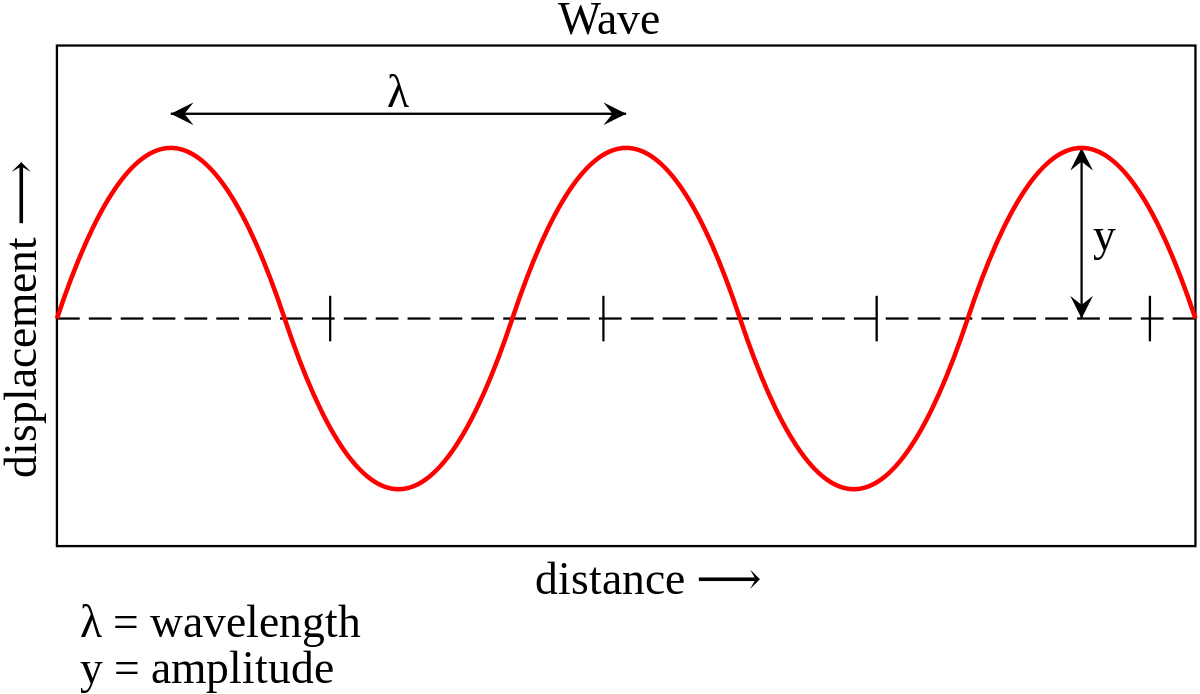
\includegraphics[scale=0.25]{baa-documentation/img/Amplitude.png}
	\caption[Amplitude and wavelength illustrated]{Amplitude and wavelength \footnotemark}
	\label{fig:Amplitude-Wavelenght}
\end{figure}
\footnotetext{\href{https://en.wikiversity.org/wiki/Amplitude}{\nolinkurl{en.wikiversity.org/wiki/Amplitude}}}

\subsection{Sampling Frequency and Resolution}
\label{sub:Sampling-Frequency-Resolution}

The sampling frequency, given in \gls{Hz}, of an audio signal, determines the resolution of the audio sample. The sampling frequency states how many samples exist for each second of the signal. Each one of these samples also has a resolution, given in bits, which determines how detailed audio waveforms are. This resolution is also referred to as bit depth. The higher the sampling rate, the higher the resolution of the signal. When recording music or many types of acoustic events, audio waveforms are typically sampled at 44.1 kHz (CD), 48 kHz, 88.2 kHz, or 96 kHz. Sampling rates higher than about 50 kHz to 60 kHz cannot supply more usable information for human listeners. Early professional audio equipment manufacturers chose sampling rates in the region of 40 to 50 kHz for this reason. 

\subsection{Tensorflow}
\label{sub:Tensorflow}

\section{Technical concepts}
\label{sec:Technical-Concepts}

In this section, technical concepts are explained in more detail, which was used in the thesis. These concepts are mostly very complex and are, therefore only touched upon so that the further conclusions of this work can be understood comprehensibly.

\subsection{Word2Vec}
\label{sub:word2wec}

\subsection{Triplet Loss}
\label{sub:Triplet-Loss}

\subsection{Mel Spectogram}
\label{sub:Mel-Spectogram}

\gls{MFCC} are

\subsection{Fourier Transformation}
\label{sub:Fourier-Transformation}

\subsubsection{Fast Fourier Transformation}
\label{subsub:Fast-Fourier-Transformation}

\subsubsection{Short Time Fourier Transformation}
\label{subsub:Short-Time-Fourier-Transformation}

\subsection{$\mu$-law Transformation}
\label{sub:Mu-Law-Transformation}

\section{Status in relation to project}
\label{sec:Status-Relation-Project}
